% Created 2022-09-28 Wed 09:37
\documentclass[9pt, b5paper]{article}
\usepackage{xeCJK}
\usepackage{minted}
\usepackage[T1]{fontenc}
\usepackage[scaled]{beraserif}
\usepackage[scaled]{berasans}
\usepackage[scaled]{beramono}
\usepackage{graphicx}
\usepackage{xcolor}
\usepackage{multirow}
\usepackage{multicol}
\usepackage{float}
\usepackage{textcomp}
\usepackage{algorithm}
\usepackage{algorithmic}
\usepackage{latexsym}
\usepackage{natbib}
\usepackage{geometry}
\geometry{left=1.2cm,right=1.2cm,top=1.5cm,bottom=1.2cm}
\newminted{common-lisp}{fontsize=\footnotesize} 
\usepackage[xetex,colorlinks=true,CJKbookmarks=true,linkcolor=blue,urlcolor=blue,menucolor=blue]{hyperref}
\author{deepwaterooo}
\date{\today}
\title{Unity Android SDK/NDK 俄罗斯方块砖3D小游戏}
\hypersetup{
  pdfkeywords={},
  pdfsubject={},
  pdfcreator={Emacs 27.1 (Org mode 8.2.7c)}}
\begin{document}

\maketitle
\tableofcontents


\section{模块搭建}
\label{sec-1}
\begin{itemize}
\item \# only inlcude two levels in TOC
\item ILRuntime的消化理解,以及与MVVM同用时的搭配理解消化
\item 热更新模块服务器模块的理解与消化搭建:
\end{itemize}

\section{把原理弄懂}
\label{sec-2}
\begin{itemize}
\item 热更新模块的实充:以前的设计模式和实现的功能还是比较完整的;现在更成熟一点儿,需要把热更新模块补充出来;
\item ILRuntime + MVVM框架设计:两者结合,前几年的时候没能把MVVM理解透彻;
\item 上次前几年主要的难点:好像是在把MVVM双向数据绑定理解得不透彻;那么这次应该就狠没有问题了,更该寻求更好的设计与解决方案
\item 性能优化:另外是对其实高级开发的越来越熟悉,希望应用的性能表现,尤其是渲染性能与速度等、这些更为高级和深入的特性成为这次二次开发的重点。

\item 现在是把自己几年前的写的游戏全忘记了,需要回去把自己的源码找出来,再读一读熟悉一下自己的源码,了解当时设计的估缺点,由此改进更将
\end{itemize}

\section{环境弄得比较好的包括:}
\label{sec-3}
\begin{itemize}
\item 输入法的搭建:终于用到了自己之前用过的好用的输入法
\item 这两天开车疲累,最迟明天中午会去南湾找房间出租,尽快解决搬家的问题;昨天晚上回来得太晚了,一路辛苦,路上只差睡着,回到家里补觉补了好多个小时。
\item 小电脑,笔记本电脑里的游戏环境搭建,今天下午去图书馆里弄(今天下午去图书馆里把需要借助快速网络来完成的事情都搭建好;家里被恶房东故意整了个腾腾慢的网,故意阻碍别人的发展,谁还愿意再这样的环境中继续住下去呢?!!!)
\end{itemize}
- 能够把程序源码读得比较懂,也并不代表把所有相关的原理就全部弄懂了;不是说还有多在的挑战,而是说要不断寻找更为有效的学习方法,快速掌握所有涉及到的相关原理;在理解得更为深入掌握了基本原理的基础上再去读源码,会不会更为有效事半功倍呢?这是一颗永远不屈服的心,爱表哥,爱生活!!!
\section{ILRuntime 库的系统再深入理解}
\label{sec-4}
\subsection{ILRuntime基本原理}
\label{sec-4-1}
\begin{itemize}
\item ILRuntime借助Mono.Cecil库来读取DLL的PE信息,以及当中类型的所有信息,最终得到方法的IL汇编码,然后通过内置的IL解译执行虚拟机来执行DLL中的代码。IL解释器代码在ILIntepreter.cs,通过Opcode来逐语句执行机器码,解释器的代码有四千多行。
\end{itemize}

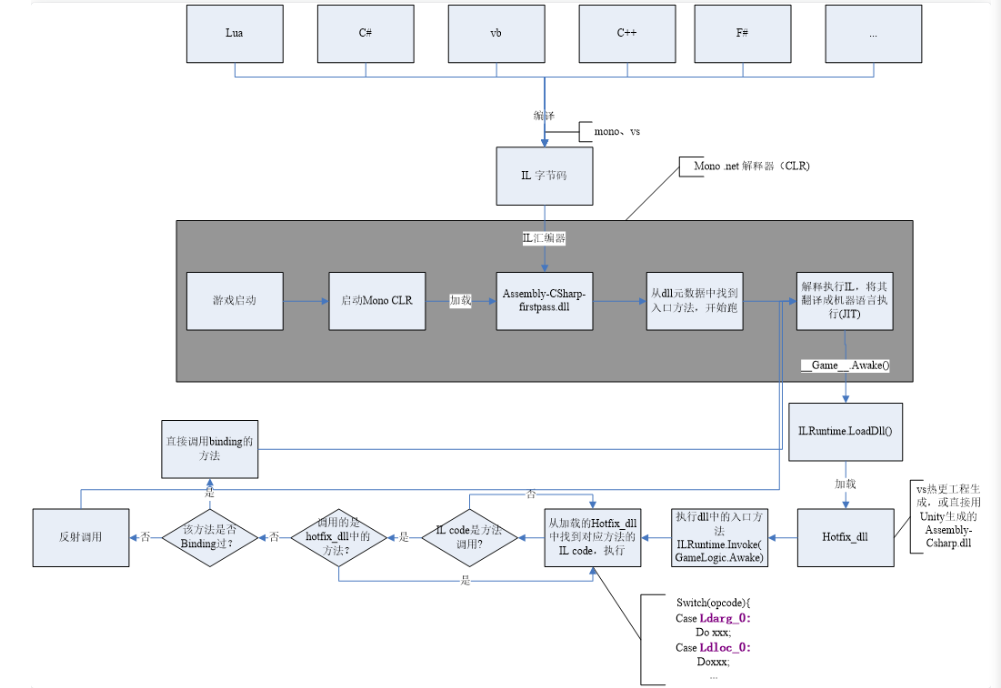
\includegraphics[width=.9\linewidth]{./pic/readme_20220926_094936.png}
\subsection{ILRuntime热更流程}
\label{sec-4-2}

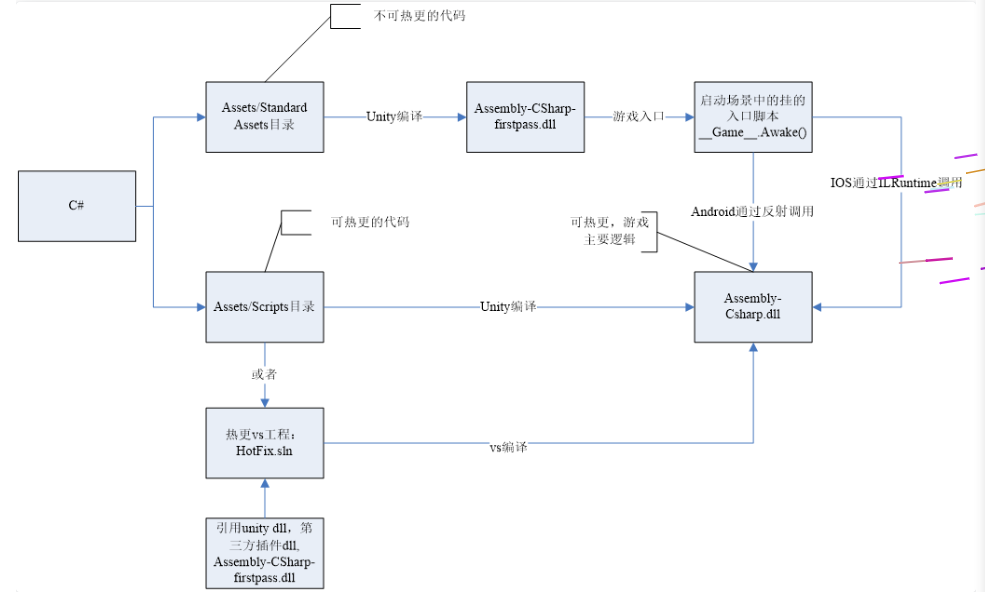
\includegraphics[width=.9\linewidth]{./pic/readme_20220926_095022.png}
\subsection{ILRuntime主要限制}
\label{sec-4-3}

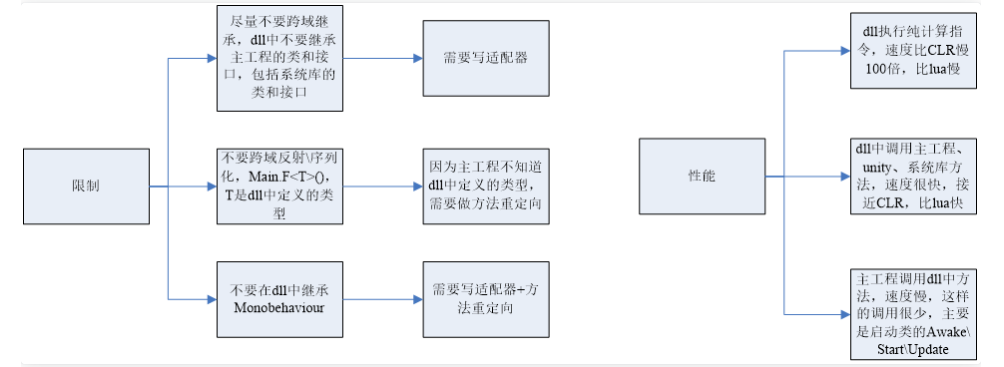
\includegraphics[width=.9\linewidth]{./pic/readme_20220926_095555.png}
\begin{itemize}
\item \textbf{委托适配器(DelegateAdapter)} :将委托实例传出给ILRuntime外部使用,将其转换成CLR委托实例。
\end{itemize}
由于IL2CPP之类的AOT编译技术无法在运行时生成新的类型,所以在创建委托实例的时候ILRuntime选择了显式注册的方式,以保证问题不被隐藏到上线后才发现。
\begin{minted}[fontsize=\scriptsize,linenos=false]{csharp}
//同一参数组合只需要注册一次
delegate void SomeDelegate(int a, float b);
Action<int, float> act;
//注册,不带返回值,最多支持五个参数传入
appDomain.DelegateManager.RegisterMethodDelegate<int, float>();

//注册,带参数返回值,最后一个参数为返回值,最多支持四个参数传入
delegate bool SomeFunction(int a, float b);
Func<int, float, bool> act;
\end{minted}
\begin{itemize}
\item \textbf{委托转换器RegisterDelegateConvertor} :需要将一个不是Action或者Func类型的委托实例传到ILRuntime外部使用,需要写委托适配器和委托转换器。委托转换器将Action和Func转换成你真正需要的那个委托类型
\end{itemize}
\begin{minted}[fontsize=\scriptsize,linenos=false]{csharp}
app.DelegateManager.RegisterDelegateConvertor<SomeFunction>((action) =>
{
    return new SomeFunction((a, b) =>
    {
       return ((Func<int, float, bool>)action)(a, b);
    });
});
\end{minted}
\begin{itemize}
\item 为了避免不必要的麻烦,以及后期热更出现问题,建议: 1、尽量避免不必要的跨域委托调用 2、尽量使用Action以及Func委托类型
\item \textbf{CLR重定向:} ILRuntime为了解决外部调用内部接口的问题,引入了CLR重定向机制。 原理就是当IL解译器发现需要调用某个指定CLR方法时,将实际调用重定向到另外一个方法进行挟持,再在这个方法中对ILRuntime的反射的用法进行处理
\item 从代码中可以看出重定向的工作是把方法挟持下来后装到ILIntepreter的解释器里面实例化
\item 不带返回值的重定向:
\end{itemize}
\begin{minted}[fontsize=\scriptsize,linenos=false]{csharp}
public static StackObject* CreateInstance(ILIntepreter intp, StackObject* esp,
                                          List<object> mStack, CLRMethod method, bool isNewObj) {
    // 获取泛型参数<T>的实际类型
    IType[] genericArguments = method.GenericArguments;
    if (genericArguments != null && genericArguments.Length == 1) {
        var t = genericArguments[0];
        if (t is ILType) { // 如果T是热更DLL里的类型 
            // 通过ILRuntime的接口来创建实例
            return ILIntepreter.PushObject(esp, mStack, ((ILType)t).Instantiate());
        } else // 通过系统反射接口创建实例
            return ILIntepreter.PushObject(esp, mStack, Activator.CreateInstance(t.TypeForCLR));
    } else
        throw new EntryPointNotFoundException();
}
// 注册
foreach (var i in typeof(System.Activator).GetMethods()) {
    // 找到名字为CreateInstance,并且是泛型方法的方法定义
    if (i.Name == "CreateInstance" && i.IsGenericMethodDefinition) {
        // RegisterCLRMethodRedirection:通过redirectMap存储键值对MethodBase-CLRRedirectionDelegate,如果i不为空且redirectMap中没有传入的MethodBase(即下方的i)则存储redirectMap[i] = CreateInstance。所以如此看来注册行为就是把键值对存储到redirectMap的过程
        appdomain.RegisterCLRMethodRedirection(i, CreateInstance);
    }
}
\end{minted}
\begin{itemize}
\item 带返回值方法的重定向
\end{itemize}
\begin{minted}[fontsize=\scriptsize,linenos=false]{csharp}
public unsafe static StackObject* DLog(ILIntepreter __intp, StackObject* __esp,
                                       List<object> __mStack, CLRMethod __method, bool isNewObj)  {
    ILRuntime.Runtime.Enviorment.AppDomain __domain = __intp.AppDomain;
    StackObject* ptr_of_this_method;
    // 只有一个参数,所以返回指针就是当前栈指针ESP - 1
    StackObject* __ret = ILIntepreter.Minus(__esp, 1);
    // 第一个参数为ESP -1, 第二个参数为ESP - 2,以此类推
    ptr_of_this_method = ILIntepreter.Minus(__esp, 1);
    // 获取参数message的值
    object message = StackObject.ToObject(ptr_of_this_method, __domain, __mStack);
    // 需要清理堆栈
    __intp.Free(ptr_of_this_method);
    // 如果参数类型是基础类型,例如int,可以直接通过int param = ptr_of_this_method->Value获取值,
    // 关于具体原理和其他基础类型如何获取,请参考ILRuntime实现原理的文档。
            
    // 通过ILRuntime的Debug接口获取调用热更DLL的堆栈
    string stackTrace = __domain.DebugService.GetStackTrance(__intp);
    Debug.Log(string.Format("{0}\n{1}", format, stackTrace));
    return __ret;
}
\end{minted}
\begin{itemize}
\item \textbf{LitJson集成}: Json序列化是开发中非常经常需要用到的功能,考虑到其通用性,因此ILRuntime对LitJson这个序列化库进行了集成
\end{itemize}
\begin{minted}[fontsize=\scriptsize,linenos=false]{csharp}
//对LitJson进行注册,需要在注册CLR绑定之前
LitJson.JsonMapper.RegisterILRuntimeCLRRedirection(appdomain);
//LitJson使用
//将一个对象转换成json字符串
string json = JsonMapper.ToJson(obj);
//json字符串反序列化成对象
JsonTestClass obj = JsonMapper.ToObject<JsonTestClass>(json);
\end{minted}
\begin{itemize}
\item \textbf{ILRuntime的性能优化}
\begin{itemize}
\item 值类型优化:使用ILRuntime外部定义的值类型(例如UnityEngine.Vector3)在默认情况下会造成额外的装箱拆箱开销。ILRuntime在1.3.0版中增加了值类型绑定(ValueTypeBinding)机制,通过对这些值类型添加绑定器,可以大幅增加值类型的执行效率,以及避免GC Alloc内存分配。
\item 大规模数值计算:如果在热更内需要进行大规模数值计算,则可以开启ILRuntime在2.0版中加入的寄存器模式来进行优化
\item 避免使用foreach:尽量避免使用foreach,会不可避免地产生GC。而for循环不会。
\item 加载dll并在逻辑后处理进行简单调用
\item 整个文件流程:创建IEnumerator并运行->用文件流判断并读入dll和pdb->尝试加载程序集dll->(如果加载成功)初始化脚本引擎(InitializeILRuntime())->执行脚本引擎加载后的逻辑处理(OnHotFixLoaded())->程序销毁(在OnDestoy中关闭dll和pdb的文件流)
\item MemoryStream:为系统提供流式读写。MemoryStream类封装一个字节数组,在构造实例时可以使用一个字节数组作为参数,但是数组的长度无法调整。使用默认无参数构造函数创建实例,可以使用Write方法写入,随着字节数据的写入,数组的大小自动调整。 参考博客:传送门
\item appdomain.LoadAssembly:将需要热更的dll加载到解释器中。第一个填入dll以及pdb,这里的pdb应该是dll对应的一些标志符号。 后面的ILRuntime.Mono.Cecil.Pdb.PdbReaderProvider()是动态修改程序集,它的作用是给ILRuntime.Mono.Cecil.Pdb.PdbReaderProvider()里的GetSymbolReader)(传入两个参数,一个是通过转化后的ModuleDefinition.ReadModule(stream(即dll))模块定义,以及原来的symbol(即pdb) GetSymbolReader主要的作用是检测其中的一些符号和标志是否为空,不为空的话就进行读取操作。 (这些内容都是ILRuntime中的文件来完成)
\end{itemize}
\item Unity MonoBehaviour lifecycle methods callback execute orders:
\item 还有一个看起来不怎么清楚的,将就凑合着看一下:这几个图因为文件地址错误丢了,改天再补一下
\item IL热更优点:
\begin{itemize}
\item 1、无缝访问C\#工程的现成代码,无需额外抽象脚本API
\item 2、直接使用VS2015进行开发,ILRuntime的解译引擎支持.Net 4.6编译的DLL
\item 3、执行效率是L\#的10-20倍
\item 4、 \textbf{选择性的CLR绑定使跨域调用更快速,绑定后跨域调用的性能能达到slua的2倍左右(从脚本调用GameObject之类的接口)}
\item 5、支持跨域继承(代码里的完美学演示)
\item 6、完整的泛型支持(代码里的完美学演示)
\item 7、拥有Visual Studio的调试插件,可以实现真机源码级调试。支持Visual Studio 2015 Update3 以及Visual Studio 2017和Visual Studio 2019
\item 8、最新的2.0版引入的寄存器模式将数学运算性能进行了大幅优化
\end{itemize}
\end{itemize}

\subsection{ILRuntime启动调试}
\label{sec-4-4}
\begin{itemize}
\item ILRuntime建议全局只创建一个AppDomain,在函数入口添加代码启动调试服务
\end{itemize}
\begin{minted}[fontsize=\scriptsize,linenos=false]{csharp}
appdomain.DebugService.StartDebugService(56000)
\end{minted}
\begin{itemize}
\item 运行主工程(Unity工程)
\item 在热更的VS工程中 点击 - 调试 - 附加到ILRuntime调试,注意使用一样的端口
\item 如果使用VS2015的话需要Visual Studio 2015 Update3以上版本
\end{itemize}
\subsection{线上项目和资料}
\label{sec-4-5}
\begin{itemize}
\item 掌趣很多项目都是使用ILRuntime开发,并上线运营,比如:真红之刃,境·界 灵压对决,全民奇迹2,龙族世界,热血足球
\item 初音未来:梦幻歌姬 使用补丁方式:\url{https://github.com/wuxiongbin/XIL}
\item 本文流程图摘自:ILRuntime的QQ群的《ILRuntime热更框架.docx》(by a 704757217)
\item Unity实现c\#热更新方案探究(三): \url{https://zhuanlan.zhihu.com/p/37375372}
\end{itemize}

\section{Framework.Core核心理解: 现在有足足的干劲把ILRuntime + MVVM热更新框架里的方方面面都理解消化透彻!爱表哥爱生活}
\label{sec-5}
\subsection{Adaptor}
\label{sec-5-1}
\subsubsection{IDisposableAdaptor : CrossBindingAdaptor}
\label{sec-5-1-1}
\begin{minted}[fontsize=\scriptsize,linenos=false]{csharp}
public class IDisposableAdaptor : CrossBindingAdaptor {
// 实现基类里所定义的三个方法    
    public override Type BaseCLRType {
        get {
            return typeof(IDisposable);
        }
    }
    public override Type AdaptorType {
        get {
            return typeof(Adaptor);
        }
    }
    public override object CreateCLRInstance(ILRuntime.Runtime.Enviorment.AppDomain appdomain, ILTypeInstance instance) {
        return new Adaptor(appdomain, instance);
    }

    internal class Adaptor : IDisposable, CrossBindingAdaptorType {
        ILTypeInstance instance; // 基类CrossBindingAdaptorType 里所必须有的一个实例
        ILRuntime.Runtime.Enviorment.AppDomain appdomain;

        public Adaptor() { }
        public Adaptor(ILRuntime.Runtime.Enviorment.AppDomain appdomain, ILTypeInstance instance) {
            this.appdomain = appdomain;
            this.instance = instance;
        }
        public ILTypeInstance ILInstance { get { return instance; } } // getter

        IMethod _Dispose;
        public void Dispose() {
            if (_Dispose == null) 
                _Dispose = instance.Type.GetMethod("Dispose", 0);
            if (_Dispose != null)
                appdomain.Invoke(_Dispose, instance);
        }
    }
}
\end{minted}
\subsubsection{IEnumeratorObjectAdaptor : CrossBindingAdaptor \{ // 叠代器适配器? 不是集合元素里轮询的叠代器,而是协程}
\label{sec-5-1-2}
\begin{minted}[fontsize=\scriptsize,linenos=false]{csharp}
public class IEnumeratorObjectAdaptor : CrossBindingAdaptor { 
// 基类里的三个方法的实现
    public override Type BaseCLRType {
        get {
            return typeof(IEnumerator<object>);
        }
    }
    public override Type AdaptorType {
        get {
            return typeof(Adaptor);
        }
    }
    public override object CreateCLRInstance(ILRuntime.Runtime.Enviorment.AppDomain appdomain, ILTypeInstance instance) {
        return new Adaptor(appdomain, instance);
    }

// 这些个IXxxxx IEnumerator<T> 之类的,是在哪里定义的,还是说是C#语言里本来就有的呢?
// 弄不明白的这些个以I打头的:都定义在plugins里的ILRuntime的包裹里,改天可以一一再看一下
    internal class Adaptor : IEnumerator<object>, CrossBindingAdaptorType {
        ILTypeInstance instance;
        ILRuntime.Runtime.Enviorment.AppDomain appdomain;

        public Adaptor() { }
        public Adaptor(ILRuntime.Runtime.Enviorment.AppDomain appdomain, ILTypeInstance instance) {
            this.appdomain = appdomain;
            this.instance = instance;
            _get_Current = instance.Type.GetMethod(".get_Current", 0);
        }

        public ILTypeInstance ILInstance { get { return instance; } } // getter

        public object Current { // 叠代器适配器所特有的方法,当前元素
            get {
                var obj = appdomain.Invoke(_get_Current, null);
                return obj;
            }
        }
// 这里的几个方法,是因为协程需要用到,所以不得不定义的吗?还有什么基类之类的吗?
        IMethod _MoveNext;
        IMethod _get_Current;
        IMethod _Reset;
        IMethod _Dispose;
        public bool MoveNext() {
            if (_MoveNext == null) 
                _MoveNext = instance.Type.GetMethod("MoveNext", 0);
            if (_MoveNext != null)
                return (bool)appdomain.Invoke(_MoveNext, instance);
            return false;
        }
        public void Reset() {
            if (_Reset == null) 
                _Reset = instance.Type.GetMethod("MoveNext", 0);
            if (_Reset != null)
                appdomain.Invoke(_Reset, instance);
        }
        public void Dispose() {
            if (_Dispose == null) 
                _Dispose = instance.Type.GetMethod("Dispose", 0);
            if (_Dispose != null)
                appdomain.Invoke(_Dispose, instance);
        }
    }
}
\end{minted}
\subsubsection{InterfaceCrossBindingAdaptor : CrossBindingAdaptor:就是实现基类里的三个方法呀}
\label{sec-5-1-3}
\begin{minted}[fontsize=\scriptsize,linenos=false]{csharp}
public class InterfaceCrossBindingAdaptor : CrossBindingAdaptor { // 就是实现基类里的三个方法呀
    public override Type BaseCLRType {
        get {
            return typeof(IEnumerator);
        }
    }
    public override Type AdaptorType {
        get {
            return typeof(IEnumeratorObjectAdaptor.Adaptor);
        }
    }
    public override object CreateCLRInstance(ILRuntime.Runtime.Enviorment.AppDomain appdomain, ILTypeInstance instance) {
        return new IEnumeratorObjectAdaptor.Adaptor(appdomain, instance);
    }
}
\end{minted}
\subsubsection{MonoBehaviourAdapter : CrossBindingAdaptor: ./Plugins/ILRuntime/Adapters包裹里的}
\label{sec-5-1-4}
\begin{minted}[fontsize=\scriptsize,linenos=false]{csharp}
// ./Plugins/ILRuntime/Adapters/MonoBehaviourAdapter.cs: 注意这个程序所在的包裹
public class MonoBehaviourAdapter : CrossBindingAdaptor {
// 实现基类里的三个抽象方法
    public override Type BaseCLRType {
        get {
            return typeof(MonoBehaviour);
        }
    }
    public override Type AdaptorType {
        get {
            return typeof(Adaptor);
        }
    }
    public override object CreateCLRInstance(ILRuntime.Runtime.Enviorment.AppDomain appdomain, ILTypeInstance instance) {
        return new Adaptor(appdomain, instance);
    }

// 为了完整实现MonoBehaviour的所有特性,这个Adapter还得扩展,这里只抛砖引玉,只实现了最常用的Awake, Start和Update
// 像我狠熟悉的安卓Activity/Fragment的生命周期有很多回调方法一样,MonoBehavior也有好几个生命周期回调方法可供实现扩展
    public class Adaptor : MonoBehaviour, CrossBindingAdaptorType {
        ILTypeInstance instance;
        ILRuntime.Runtime.Enviorment.AppDomain appdomain;

        public Adaptor() { }
        public Adaptor(ILRuntime.Runtime.Enviorment.AppDomain appdomain, ILTypeInstance instance) {
            this.appdomain = appdomain;
            this.instance = instance;
        }
        public ILTypeInstance ILInstance { get { return instance; } set { instance = value; } }
        public ILRuntime.Runtime.Enviorment.AppDomain AppDomain { get { return appdomain; } set { appdomain = value; } }

// Awake() Start() Update() 三个生命周期架设方法的跨域适配
        IMethod mAwakeMethod;
        bool mAwakeMethodGot;
        public void Awake() {
            // Unity会在ILRuntime准备好这个实例前调用Awake,所以这里暂时先不掉用
            if (instance != null) {
                if (!mAwakeMethodGot) {
                    mAwakeMethod = instance.Type.GetMethod("Awake", 0);
                    mAwakeMethodGot = true;
                }
                if (mAwakeMethod != null) {
                    appdomain.Invoke(mAwakeMethod, instance, null);
                }
            }
        }
        IMethod mStartMethod;
        bool mStartMethodGot;
        void Start() {
            if (!mStartMethodGot) {
                mStartMethod = instance.Type.GetMethod("Start", 0);
                mStartMethodGot = true;
            }
            if (mStartMethod != null) {
                appdomain.Invoke(mStartMethod, instance, null);
            }
        }
        IMethod mUpdateMethod;
        bool mUpdateMethodGot;
        void Update() {
            if (!mUpdateMethodGot) {
                mUpdateMethod = instance.Type.GetMethod("Update", 0);
                mUpdateMethodGot = true;
            }
            if (mStartMethod != null) {
                appdomain.Invoke(mUpdateMethod, instance, null);
            }
        }
        
        public override string ToString() {
            IMethod m = appdomain.ObjectType.GetMethod("ToString", 0);
            m = instance.Type.GetVirtualMethod(m);
            if (m == null || m is ILMethod) {
                return instance.ToString();
            } else
                return instance.Type.FullName;
        }
    }
}
\end{minted}
\subsection{Factory: 顾名思义,就是工厂模式,负责生产各种不同类型的实例(生产人质)}
\label{sec-5-2}
\subsubsection{enum FactoryType}
\label{sec-5-2-1}
\begin{minted}[fontsize=\scriptsize,linenos=false]{csharp}
public enum FactoryType {
    Singleton,
    Transient,
    Pool
}
\end{minted}
\subsubsection{interface IObjectFactory}
\label{sec-5-2-2}
\begin{minted}[fontsize=\scriptsize,linenos=false]{csharp}
public interface IObjectFactory {
    object AcquireObject(string classFullName);
    void ReleaseObject(object obj);
}
\end{minted}
\subsubsection{PoolObjectFactory : Singleton<PoolObjectFactory>, IObjectFactory:单例对象池:结合工厂模式使用}
\label{sec-5-2-3}
\begin{minted}[fontsize=\scriptsize,linenos=false]{csharp}
// 单例对象池:结合工厂模式使用;现接触过的对象池包括 ThreadPool, ObjectPool, 
public class PoolObjectFactory : Singleton<PoolObjectFactory>, IObjectFactory {

    public class ObjectPool {
        public readonly List<PoolData> _pool; // readonly
        public int Max { // 该对象池储存数据上限
            get;
            set;
        }
        public bool Limit { // 该对象池设限了吗?
            get;
            set;
        }
        public ObjectPool() {
            Limit = false;
            _pool = new List<PoolData>();
        }
    }
    public class PoolData {
        public bool InUse {
            get;
            set;
        }
        public object Obj {
            get;
            set;
        }
    }
// 这里,每种类型对应一个对象池(因为每种类型根据游戏需要可能初始化数量等不同有不同的要求),用一个字典管理不同类型的对象池
    private readonly Dictionary<Type, ObjectPool> pool;
    public PoolObjectFactory() {
        pool = new Dictionary<Type, ObjectPool>();
    }

    public object AcquireObject(string classFullName) {
        Type type = GameApplication.Instance.HotFix.LoadType(classFullName);
        lock (pool) { // 这里需要上锁
            if (pool.ContainsKey(type)) {
                if (pool[type]._pool.Count > 0) {
                    for (int i = 0; i < pool[type]._pool.Count; i++) {
                        var p = pool[type]._pool[i];
                        if (!p.InUse) { // 从该类型对象池里的现有对象链表中遍历出第一个没被使用的对象拿来用
                            p.InUse = true;
                            return p.Obj;
                        }
                    }
                }
                // 该类型对象池数量已经达到了上限
                if (pool[type].Limit && pool[type]._pool.Count >= pool[type].Max) 
                    throw new Exception("max limit is arrived.");
            }
            object obj = GameApplication.Instance.HotFix.CreateInstance(classFullName);
            var poolData = new PoolData {
                InUse = true,
                Obj = obj
            };
            if (!pool.ContainsKey(type)) {
                ObjectPool objPool = new ObjectPool();
                pool.Add(type, objPool);
            }
            pool[type]._pool.Add(poolData);
            return obj;
        }
    }
    public void ReleaseObject(object obj) { }
}
\end{minted}
\subsubsection{SingletonObjectFactory : IObjectFactory: 单例对象工厂}
\label{sec-5-2-4}
\begin{minted}[fontsize=\scriptsize,linenos=false]{csharp}
// 单例对象工厂
public class SingletonObjectFactory : IObjectFactory {

    private static Dictionary<Type, object> cachedObjects = null;
    private static readonly object _lock = new object();

    private Dictionary<Type, object> CachedObjects {
        get {
            lock (_lock) {
                if (cachedObjects == null) 
                    cachedObjects = new Dictionary<Type, object>();
                return cachedObjects;
            }
        }
    }
    public object AcquireObject(string classFullName) {
        Type type = GameApplication.Instance.HotFix.LoadType(classFullName);
        if (CachedObjects.ContainsKey(type)) 
            return CachedObjects[type];
        lock (_lock) {
            var instance = GameApplication.Instance.HotFix.CreateInstance(classFullName);
            CachedObjects.Add(type, instance);
            return instance;
        }
    }
    public void ReleaseObject(object obj) { }
}
\end{minted}
\subsubsection{TransientObjectFactory : IObjectFactory}
\label{sec-5-2-5}
\begin{minted}[fontsize=\scriptsize,linenos=false]{csharp}
public class TransientObjectFactory : IObjectFactory {

    public object AcquireObject(string classFullName) {
        var instance = GameApplication.Instance.HotFix.CreateInstance(classFullName);
        return instance;
    }
    public void ReleaseObject(object obj) { }
}
\end{minted}
\subsection{Inject: 美其名曰(自动)注入的背后,都是强大优化过的逻辑在支撑!爱表哥,爱生活}
\label{sec-5-3}
\subsubsection{ServiceLocatorContain}
\label{sec-5-3-1}
\begin{minted}[fontsize=\scriptsize,linenos=false]{csharp}
public class ServiceLocatorContain {
    public string TypeName {
        get;
        private set;
    }
    public Func<object> Function {
        get;
        set;
    }
    public ServiceLocatorContain(string name, Func<object> func) {
        TypeName = name;
        Function = func;
    }
}
// 对象定位(创建)工厂:要么去对象池里抓一下;(当没有或是所有对象均在用且达上限)要么创建一个新的
public class ServiceLocator {
    private static readonly Dictionary<Type, ServiceLocatorContain> Container = new Dictionary<Type, ServiceLocatorContain>();

    // 两种不同类型的工厂以及对象的定位方法(每种类型提供两种不同参数的定位方法)
    private SingletonObjectFactory _singletonObjectFactory = new SingletonObjectFactory();
    private TransientObjectFactory _transientObjectFactory = new TransientObjectFactory();

    // 两种不同类型的工厂以及对象的定位方法(每种类型提供两种不同参数的定位方法)
    public void RegisterSingleton(string interfaceName, string typeName) {
        ServiceLocatorContain contain = new ServiceLocatorContain(typeName, Lazy(FactoryType.Singleton, typeName));
        Type type = GameApplication.Instance.HotFix.LoadType(interfaceName);
        if (!Container.ContainsKey(type)) {
            Container.Add(type, contain);
        } else {
            throw new Exception("Container contains key: " + type);
        }
    }
    public void RegisterSingleton(string typeName) {
        ServiceLocatorContain contain = new ServiceLocatorContain(typeName, Lazy(FactoryType.Singleton, typeName));
        Type type = GameApplication.Instance.HotFix.LoadType(typeName);
        if (!Container.ContainsKey(type)) {
            Container.Add(type, contain);
        } else {
            throw new Exception("Container contains key: " + type);
        }
    }
    public void RegisterTransient(string interfaceName, string typeName) {
        ServiceLocatorContain contain = new ServiceLocatorContain(typeName, Lazy(FactoryType.Transient, typeName));
        Type type = GameApplication.Instance.HotFix.LoadType(interfaceName);
        if (!Container.ContainsKey(type)) {
            Container.Add(type, contain);
        } else {
            throw new Exception("Container contains key: " + type);
        }
    }
    public void RegisterTransient(string typeName) {
        ServiceLocatorContain contain = new ServiceLocatorContain(typeName, Lazy(FactoryType.Transient, typeName));
        Type type = GameApplication.Instance.HotFix.LoadType(typeName);
        if (!Container.ContainsKey(type)) {
            Container.Add(type, contain);
        } else {
            throw new Exception("Container contains key: " + type);
        }
    }

    public void Clear() {
        Container.Clear();
    }
    public TInterface Resolve<TInterface>(string keyName) where TInterface : class {
        return Resolve(GameApplication.Instance.HotFix.LoadType(keyName)) as TInterface;
    }
    private static object Resolve(Type type) {
        if (!Container.ContainsKey(type)) 
            return null;
        return Container[type].Function();
    }
    private Func<object> Lazy(FactoryType factoryType, string typeFullName) {
        return () => {
            switch (factoryType) {
            case FactoryType.Singleton:
                return _singletonObjectFactory.AcquireObject(typeFullName);
            default:
                return _transientObjectFactory.AcquireObject(typeFullName);
            }
        };
    }
}
\end{minted}
\subsection{Wrap}
\label{sec-5-4}
\subsection{GameApplication: 游戏入口类}
\label{sec-5-5}
\begin{minted}[fontsize=\scriptsize,linenos=false]{csharp}
// 游戏入口类
public class GameApplication : MonoBehaviour {
    private const string TAG = "GameApplication";
        
    private static GameApplication _instance;
    public static GameApplication Instance {
        get {
            return _instance;
        }
    }
    public IHotFixMain HotFix {
        get;
        set;
    }

// 五个用户、客户端可配置变量,以及它们的根据用户配置(读取系统中用户配置文件里的相关五个配置)
    // 是否使用PDB调试信息
    public bool usePDB = false;
    // 是否使用ILRuntime模式热更新
    public bool useILRuntime = false;
    // 是否使用本地资源
    public bool useLocal = false;
    // 资源服务器路径
    public string webRoot = string.Empty;
    // 强制登录
    public bool forceLogin = false;
    
    public ScreenRaycaster ScreenRaycaster {
        get;
        private set;
    }
// 这个公用方法应该是跟游戏中时常需要接入一个或是多个游戏SDK相关,提供便利接入方法
    public ShareSDK ShareSDK { 
        get;
        private set;
    }
    void Awake() {
        _instance = this;
        ScreenRaycaster = GameObject.Find("Gestures").GetComponent<ScreenRaycaster>();
        DontDestroyOnLoad(gameObject); // <<<<<<<<<<<<<<<<<<<< 我自己的游戏中实现过这个,可是现在回想得好辛苦呀。。。爱表哥爱生活爱游戏
        //InitializeClientConfig();
        //InitializeSDKs();
        CoroutineHelper.StartCoroutine(Initialize()); // 协程:
#region TestSamples
        //FingerEventTemp.Instance.RegisterGestureEvents();
        //TestNTS.Instance.TestLinesAngle();
        //GeometryManager.Instance.Test();
#endregion
    }
// 客户端的配置是写在一个文件里的,需要的话直接读就可以了,安卓系统很多地方也这样
    void InitializeClientConfig() {
        var str = FileHelp.ReadString("ClientConfig.txt"); 
        if (!string.IsNullOrEmpty(str)) {
            JsonObject jsonObject = JsonSerializer.Deserialize(str) as JsonObject;
            if (jsonObject != null) {
                if (jsonObject.ContainsKey("usePDB")) 
                    usePDB = (bool)jsonObject["usePDB"];
                if (jsonObject.ContainsKey("useILRuntime")) 
                    usePDB = (bool)jsonObject["useILRuntime"];
                if (jsonObject.ContainsKey("useLocal")) 
                    usePDB = (bool)jsonObject["useLocal"];
                if (jsonObject.ContainsKey("webRoot")) 
                    ResourceConstant.ResourceWebRoot = jsonObject["webRoot"].ToString();
                if (jsonObject.ContainsKey("forceLogin")) 
                    forceLogin = (bool)jsonObject["forceLogin"];
            }
        }
    }

    void InitializeSDKs() {
        if (Application.platform == RuntimePlatform.IPhonePlayer || Application.platform == RuntimePlatform.Android) 
            InitializeShareSDK();
    }
    void InitializeShareSDK() {
        ShareSDK = GetComponent<ShareSDK>();
        ShareSDK.authHandler = AuthResultHandler;
        ShareSDK.Authorize(PlatformType.WeChat);
    }
    // ShareSDK执行授权回调
    void AuthResultHandler(int reqID, ResponseState state, PlatformType type, Hashtable result) {
        if (state == ResponseState.Success) {
            Debug.Log("ShareSDK authorize success!");
        } else if (state == ResponseState.Fail) {
            Debug.Log("fail! error code = " + result["error_code"] + "; error msg = " + result["error_msg"]);
        } else if (state == ResponseState.Cancel) {
            Debug.Log("cancel!");
        }
    }

// 协程是说:游戏启动时,给这个控件(gameObject)加载运行时元件ResourceMap(本质上是个脚本程序); 加载完毕自动触发StartHotFix()函数热更新回调
    IEnumerator Initialize() { 
        ResourceMap resourceMap = gameObject.AddComponent<ResourceMap>();
        resourceMap.OnInitializeSuccess += StartHotFix;
        ResourceConstant.Loader = resourceMap;
        yield return new WaitForEndOfFrame();
    }
    public void StartHotFix() {
        Debug.Log(TAG + ": StartHotFix()");
        Debug.Log(TAG + " useILRuntime: " + useILRuntime); 
        if (Application.platform == RuntimePlatform.IPhonePlayer) {
            HotFix = HotFixILRunTime.Instance;
        } else {
            if (useILRuntime) { // 使用热更新程序集的实例
                HotFix = HotFixILRunTime.Instance;
            } else { // 这里是,还需要再理解消化一下
                HotFix = HotFixReflector.Instance;
            }
        }
    }
}
\end{minted}

\subsection{HotFixILRunTime : SingletonMono<HotFixILRunTime>, IHotFixMain: 因为跨域交互,所以即使是热更新包,也继承自unity MonoBehaviour}
\label{sec-5-6}
\begin{minted}[fontsize=\scriptsize,linenos=false]{csharp}
public class HotFixILRunTime : SingletonMono<HotFixILRunTime>, IHotFixMain { // SingletonMono<T> where T : MonoBehaviour帮助类里有定义
    public static ILRuntime.Runtime.Enviorment.AppDomain appDomain;

    void Start() {
        appDomain = new ILRuntime.Runtime.Enviorment.AppDomain();
#if UNITY_EDITOR
        appDomain.UnityMainThreadID = System.Threading.Thread.CurrentThread.ManagedThreadId;
#endif
        // 调用资源管理器加载这两个程序集:HotFix.dll + HotFix.pdb
        TextAsset dllAsset = ResourceConstant.Loader.LoadAsset<TextAsset>("HotFix.dll", "HotFix.dll"); // 同步加载
        var msDll = new System.IO.MemoryStream(dllAsset.bytes); // 这里涉及到内存管理吗?以前我不曾涉及,现在长大了,应该把它理解消化好
        if (GameApplication.Instance.usePDB) {
            ResourceConstant.Loader.LoadAssetAsyn<TextAsset>("HotFix.pdb", "HotFix.pdb", (pdbAsset) => { // 异步加载
                var msPdb = new System.IO.MemoryStream(pdbAsset.bytes);
                appDomain.LoadAssembly(msDll, msPdb, new Mono.Cecil.Mdb.MdbReaderProvider());
                StartApplication(); // <<<<<<<<<<<<<<<<<<<< 
            }, EAssetBundleUnloadLevel.ChangeSceneOver);
        } else {
            appDomain.LoadAssembly(msDll, null, new Mono.Cecil.Mdb.MdbReaderProvider());
            StartApplication();
        }
    }
    void StartApplication() {
        InitializeILRunTimeHotFixSetting();
        DoStaticMethod("HotFix.HotFixMain", "Start");
    }
    void InitializeILRunTimeHotFixSetting() {
        InitializeDelegateSetting(); // 方法被我搬到了文件的最后,太长比较简单
        InitializeCLRBindSetting();
        InitializeAdapterSetting();
        InitializeValueTypeSetting();
    }
    unsafe void InitializeCLRBindSetting() {
        foreach (var i in typeof(System.Activator).GetMethods()) {
            // 找到名字为CreateInstance,并且是泛型方法的方法定义 ?
            if (i.Name == "CreateInstance" && i.IsGenericMethodDefinition) 
                appDomain.RegisterCLRMethodRedirection(i, CreateInstance); // 方法重定向?再理解消化一下,不太懂还
        }
    }

    void InitializeAdapterSetting() {
        appDomain.RegisterCrossBindingAdaptor(new ViewModelBaseAdapter());  
        appDomain.RegisterCrossBindingAdaptor(new UnityGuiViewAdapter());   
        appDomain.RegisterCrossBindingAdaptor(new ModuleBaseAdapter());     
        appDomain.RegisterCrossBindingAdaptor(new IEnumeratorObjectAdaptor()); // 协程适配
        appDomain.RegisterCrossBindingAdaptor(new MonoBehaviourAdapter()); // <<<<<<<<<<<<<<<<<<<< 临时补了一下,也有了
        appDomain.RegisterCrossBindingAdaptor(new InterfaceCrossBindingAdaptor());
    }
    void InitializeValueTypeSetting() {
        appDomain.RegisterValueTypeBinder(typeof(Vector3), new Vector3Binder());
        appDomain.RegisterValueTypeBinder(typeof(Vector2), new Vector2Binder());
        appDomain.RegisterValueTypeBinder(typeof(Quaternion), new QuaternionBinder());
    }

// 定义如何调用热更新程序集里的静态入口方法
    object DoStaticMethod(string type, string method) { 
        var hotfixType = appDomain.GetType(type);
        var staticMethod = hotfixType.GetMethod(method, 0);
        return appDomain.Invoke(staticMethod, null, null);
    }

// 定义热更新的两个方法的特用实现    
#region Override
    public Type LoadType(string typeName) {
        if (appDomain.LoadedTypes.ContainsKey(typeName)) {
            return appDomain.LoadedTypes[typeName].ReflectionType;
        }
        return null;
    }
    public object CreateInstance(string typeName) {
        ILType type = (ILType)appDomain.LoadedTypes[typeName];
        var instance = type.Instantiate();
        return instance;
    }
#endregion

    // 公用静态方法的实现
    public unsafe static StackObject* CreateInstance(ILIntepreter intp, StackObject* esp, IList<object> mStack, CLRMethod method, bool isNewObj) {
        // 获取泛型参数<T>的实际类型
        IType[] genericArguments = method.GenericArguments;
        if (genericArguments != null && genericArguments.Length == 1) {
            var t = genericArguments[0];
            if (t is ILType)// 如果T是热更DLL里的类型 {
                // 通过ILRuntime的接口来创建实例
                return ILIntepreter.PushObject(esp, mStack, ((ILType)t).Instantiate());
        } else
            return ILIntepreter.PushObject(esp, mStack, Activator.CreateInstance(t.TypeForCLR));// 通过系统反射接口创建实例
    } else
          throw new EntryPointNotFoundException();
}

// 不难猜测理解:所有需要热更新的方法类型(以不同的参数类型以及返回类型作区分),都要在这里向程序集的代理管理器注册相关方法回调代理    
// 同一参数组合只需要注册一次
    void InitializeDelegateSetting() { // 注册,不带返回值,最多支持五个参数传入; 注册,带参数返回值,最后一个参数为返回值,最多支持四个参数传入 ?
        appDomain.DelegateManager.RegisterMethodDelegate<int>();
        appDomain.DelegateManager.RegisterFunctionDelegate<int, string>();
        appDomain.DelegateManager.RegisterMethodDelegate<string>();
        appDomain.DelegateManager.RegisterMethodDelegate<int, int>();
        appDomain.DelegateManager.RegisterMethodDelegate<List<int>, List<int>>();
        appDomain.DelegateManager.RegisterMethodDelegate<string, string>();
        appDomain.DelegateManager.RegisterMethodDelegate<object, MessageArgs<object>>();
        appDomain.DelegateManager.RegisterMethodDelegate<object, MessageArgs<ILTypeInstance>>();
        appDomain.DelegateManager.RegisterMethodDelegate<GameObject>();
        appDomain.DelegateManager.RegisterMethodDelegate<UnityEngine.Networking.UnityWebRequest>();
        appDomain.DelegateManager.RegisterMethodDelegate<TMP_FontAsset>();
        appDomain.DelegateManager.RegisterMethodDelegate<Font>();
        appDomain.DelegateManager.RegisterMethodDelegate<AnimationClip>();
        appDomain.DelegateManager.RegisterMethodDelegate<AnimatorOverrideController>();
        appDomain.DelegateManager.RegisterMethodDelegate<RuntimeAnimatorController>();
        appDomain.DelegateManager.RegisterMethodDelegate<AudioClip>();
        appDomain.DelegateManager.RegisterMethodDelegate<Material>();
        appDomain.DelegateManager.RegisterMethodDelegate<TextAsset>();
        appDomain.DelegateManager.RegisterMethodDelegate<Sprite>();
        appDomain.DelegateManager.RegisterMethodDelegate<Texture2D>();
        appDomain.DelegateManager.RegisterMethodDelegate<TapGesture>();
        appDomain.DelegateManager.RegisterMethodDelegate<LongPressGesture>();
        appDomain.DelegateManager.RegisterMethodDelegate<DragGesture>();
        appDomain.DelegateManager.RegisterMethodDelegate<PinchGesture>();
        appDomain.DelegateManager.RegisterMethodDelegate<Exception>();
        appDomain.DelegateManager.RegisterFunctionDelegate<GameObject, GameObject>();
        appDomain.DelegateManager.RegisterFunctionDelegate<ILTypeInstance, ILTypeInstance, int>();
// 在Unity的程序集与热更新的程序集跨域之间,这里给出了方法代理转换的实现逻辑,几座小桥流水人家,爱表哥爱生活
// 委托转换器:需要将一个不是Action或者Func类型的委托实例传到ILRuntime外部使用,需要写委托适配器和委托转换器。
// 委托转换器将Action和Func转换成你真正需要的那个委托类型
// 为了避免不必要的麻烦,以及后期热更出现问题,建议: 1、尽量避免不必要的跨域委托调用 2、尽量使用Action以及Func委托类型
        appDomain.DelegateManager.RegisterDelegateConvertor<UnityAction>((action) => {
            return new UnityAction(() => {
                ((Action)action)();
            });
        });
        appDomain.DelegateManager.RegisterDelegateConvertor<UnityAction<bool>>((action) => {
            return new UnityAction<bool>((b) => {
                ((Action<bool>)action)(b);
            });
        });
        appDomain.DelegateManager.RegisterDelegateConvertor<UnityAction<int>>((action) => {
            return new UnityAction<int>((b) => {
                ((Action<int>)action)(b);
            });
        });
        appDomain.DelegateManager.RegisterDelegateConvertor<UnityAction<long>>((action) => {
            return new UnityAction<long>((b) => {
                ((Action<long>)action)(b);
            });
        });
        appDomain.DelegateManager.RegisterDelegateConvertor<UnityAction<float>>((action) => {
            return new UnityAction<float>((b) => {
                ((Action<float>)action)(b);
            });
        });
        appDomain.DelegateManager.RegisterDelegateConvertor<UnityAction<string>>((action) => {
            return new UnityAction<string>((b) => {
                ((Action<string>)action)(b);
            });
        });
        appDomain.DelegateManager.RegisterDelegateConvertor<UnityAction<BaseEventData>>((action) => {
            return new UnityAction<BaseEventData>((b) => {
                ((Action<BaseEventData>)action)(b);
            });
        });
        appDomain.DelegateManager.RegisterDelegateConvertor<GestureRecognizerTS<TapGesture>.GestureEventHandler>((action) => {
            return new GestureRecognizerTS<TapGesture>.GestureEventHandler((gesture) => {
                ((Action<TapGesture>)action)(gesture);
            });
        });
        appDomain.DelegateManager.RegisterDelegateConvertor<GestureRecognizerTS<LongPressGesture>.GestureEventHandler>((action) => {
            return new GestureRecognizerTS<LongPressGesture>.GestureEventHandler((gesture) => {
                ((Action<LongPressGesture>)action)(gesture);
            });
        });
        appDomain.DelegateManager.RegisterDelegateConvertor<GestureRecognizerTS<DragGesture>.GestureEventHandler>((action) => {
            return new GestureRecognizerTS<DragGesture>.GestureEventHandler((gesture) => {
                ((Action<DragGesture>)action)(gesture);
            });
        });
        appDomain.DelegateManager.RegisterDelegateConvertor<GestureRecognizerTS<PinchGesture>.GestureEventHandler>((action) => {
            return new GestureRecognizerTS<PinchGesture>.GestureEventHandler((gesture) => {
                ((Action<PinchGesture>)action)(gesture);
            });
        });
        #if UNITY_IPHONE
                appDomain.DelegateManager.RegisterDelegateConvertor<com.mob.FinishedRecordEvent>((action) => {
            return new com.mob.FinishedRecordEvent((ex) => {
                ((Action<Exception>)action)(ex);
            });
        });
        #endif
        appDomain.DelegateManager.RegisterDelegateConvertor<Comparison<ILTypeInstance>>((action) => {
            return new Comparison<ILTypeInstance>((x, y) => {
                return ((Func<ILTypeInstance, ILTypeInstance, System.Int32>)action)(x, y);
            });
        });
    }
}
\end{minted}
\subsection{HotFixReflector : SingletonMono<HotFixReflector>, IHotFixMain}
\label{sec-5-7}
\begin{minted}[fontsize=\scriptsize,linenos=false]{csharp}
public class HotFixReflector : SingletonMono<HotFixReflector>, IHotFixMain {
    public static Assembly assembly;

    void Start() {
        ResourceConstant.Loader.LoadAssetAsyn<TextAsset>( // 这里说是异步加载
            "HotFix.dll", "HotFix.dll",
            LoadHotFixDllSuccess,
            EAssetBundleUnloadLevel.ChangeSceneOver);
    }

    void LoadHotFixDllSuccess(TextAsset dllAsset) {
        if (GameApplication.Instance.usePDB) {
            ResourceConstant.Loader.LoadAssetAsyn<TextAsset>( // 同样是异步加载
                "HotFix.pdb",
                "HotFix.pdb", (pdbAsset) => {
                    assembly = Assembly.Load(dllAsset.bytes, pdbAsset.bytes);
                    StartApplication(); // <<<<<<<<<< 
                }, EAssetBundleUnloadLevel.ChangeSceneOver);
        } else {
            assembly = AppDomain.CurrentDomain.Load(dllAsset.bytes);
            StartApplication();
        }
    }
    
    void StartApplication() {
        try {
            Type hotfixMainType = assembly.GetType("HotFix.HotFixMain");
            MethodInfo startMethod = hotfixMainType.GetMethod("Start");
            startMethod.Invoke(null, null);
        } catch (Exception e) {
            string errorMessage = string.Empty;
            if (e.InnerException != null) 
                errorMessage = e.InnerException.Message + e.InnerException.StackTrace;
            else errorMessage = e.Message + e.StackTrace;
            DebugHelper.LogError(errorMessage, true);
        }
    }
#region Override
    public Type LoadType(string typeName) {
        Type type = assembly.GetTypes().FirstOrDefault(t => t.FullName == typeName);
        if (type == null) {
            DebugHelper.LogError(string.Format("Cant't find Class by class name:'{0}'", typeName), true);
            throw new Exception(string.Format("Cant't find Class by class name:'{0}'", typeName));
        }
        return type;
    }
    public object CreateInstance(string typeName) {
        return Activator.CreateInstance(LoadType(typeName));
    }
#endregion
}
\end{minted}
\subsection{IHotFixMain interface}
\label{sec-5-8}
\begin{minted}[fontsize=\scriptsize,linenos=false]{csharp}
public interface IHotFixMain {
    Type LoadType(string typeName);
    object CreateInstance(string typeName);
}
\end{minted}

\section{Framework.MVVM: Unity中定义好的MVVM架构;使用ILRuntime定义实现了必要的跨域跨程序集适配,以及数据观察回调等}
\label{sec-6}
\subsection{DataBinding: MVVM具备双向数据绑定功能;这里这个框架里通过代理观察者模式来实现数据的改变通知与回调}
\label{sec-6-1}
\subsubsection{BindableProperty<T> : 泛型基类,可绑定的属性}
\label{sec-6-1-1}
\begin{minted}[fontsize=\scriptsize,linenos=false]{csharp}
public class BindableProperty<T> { // 泛型基类
    private T _value;

    public Action<T, T> OnValueChanged; // 代理模式,观察者模式?
    public T Value {
        get {
            return _value;
        }
        set {
            if (!Equals(_value, value)) {
                T old = _value;
                _value = value;
                ValueChanged(old, _value);
            }
        }
    }
    void ValueChanged(T oldValue, T newValue) {
        if (OnValueChanged != null) 
            OnValueChanged(oldValue, newValue);
    }

    public override string ToString() {
        return (Value != null ? Value.ToString() : "null");
    }
}
\end{minted}
\subsubsection{ObservableList<T> : IList<T> :可被观察的链表,同样包装成泛型基类}
\label{sec-6-1-2}
\begin{minted}[fontsize=\scriptsize,linenos=false]{csharp}
public class ObservableList<T> : IList<T> { // 可被观察的链表:同样包装成泛型基类

    public Action<List<T>, List<T>> OnValueChanged;
    public Action<T> OnAdd;
    public Action<int, T> OnInsert;
    public Action<T> OnRemove;
    private List<T> _value = new List<T>(); // <<<<<<<<<< 

    public List<T> Value {
        get {
            return _value;
        }
        set {
            if (!Equals(_value, value)) {
                var old = _value;
                _value = value;
                ValueChanged(old, _value);
            }
        }
    }
    void ValueChanged(List<T> oldValue, List<T> newValue) {
        if (OnValueChanged != null) 
            OnValueChanged(oldValue, newValue);
    }

    public IEnumerator<T> GetEnumerator() {
        return _value.GetEnumerator();
    }
    IEnumerator IEnumerable.GetEnumerator() {
        return GetEnumerator();
    }

// 覆写和定义链表的相关必要方法
    public void Add(T item) {
        _value.Add(item);
        if (OnAdd != null) 
            OnAdd(item);
    }
    public void Clear() {
        _value.Clear();
    }
    public bool Contains(T item) {
        return _value.Contains(item);
    }
    public void CopyTo(T[] array, int arrayIndex) {
        _value.CopyTo(array, arrayIndex);
    }
    public bool Remove(T item) {
        if (_value.Remove(item)) {
            if (OnRemove != null) 
                OnRemove(item);
            return true;
        }
        return false;
    }
    public int Count {
        get {
            return _value.Count;
        }
    }
    public bool IsReadOnly {
        get;
        private set;
    }
    public int IndexOf(T item) {
        return _value.IndexOf(item);
    }
    public void Insert(int index, T item) {
        _value.Insert(index, item);
        if (OnInsert != null) {
            OnInsert(index, item);
        }
    }
    public void RemoveAt(int index) {
        _value.RemoveAt(index);
    }
    public T this[int index] {
        get {
            return _value[index];
        }
        set {
            _value[index] = value;
        }
    }
}
\end{minted}
\subsubsection{PropertyBinder<ViewModelBase>: ViewModel(的基类以及继承类)的绑定辅助相关方法定义类}
\label{sec-6-1-3}
\begin{minted}[fontsize=\scriptsize,linenos=false]{csharp}
// ViewModel(的基类以及继承类)的绑定辅助相关方法定义类
public class PropertyBinder<ViewModelBase> { 

    private delegate void BindHandler(ViewModelBase viewModel); // 这里才真正意义上的代理模式吧
    private delegate void UnBindHandler(ViewModelBase viewModel);

    private readonly List<BindHandler> binders = new List<BindHandler>();
    private readonly List<UnBindHandler> unBinders = new List<UnBindHandler>();

    public void Add<TProperty>(string name, string realTypeName, Action<TProperty, TProperty> valueChangedHandler) {
        var fieldInfo = GameApplication.Instance.HotFix.LoadType(realTypeName).GetField(name, BindingFlags.Instance | BindingFlags.Public);
        if (fieldInfo == null) 
            throw new Exception(string.Format("Unable to find bindableproperty field '{0}.{1}'", realTypeName, name));
        binders.Add(viewModel => {
            GetPropertyValue<TProperty>(name, viewModel, realTypeName, fieldInfo).OnValueChanged += valueChangedHandler;
        });
        unBinders.Add(viewModel => {
            GetPropertyValue<TProperty>(name, viewModel, realTypeName, fieldInfo).OnValueChanged -= valueChangedHandler;
        });
    }
    private BindableProperty<TProperty> GetPropertyValue<TProperty>(string name, ViewModelBase viewModel,
                                                                    string realTypeName, FieldInfo fieldInfo) {
        var value = fieldInfo.GetValue(viewModel);
        BindableProperty<TProperty> bindableProperty = value as BindableProperty<TProperty>;
        if (bindableProperty == null) 
            throw new Exception(string.Format("Illegal bindableproperty field '{0}.{1}' ", realTypeName, name));
        return bindableProperty;
    }

// 这里告诉一个常识说:任何一个ViewModel,不管是蕨类还是继承后的子类,它们都有可能有好几个视图与其绑定
    public void Bind(ViewModelBase viewModel) {
        if (viewModel != null) 
            for (int i = 0; i < binders.Count; i++) 
                binders[i](viewModel);
    }
// 这里告诉一个常识说:任何一个ViewModel,不管是蕨类还是继承后的子类,它们都有可能有好几个视图,需要与其解绑定
    public void UnBind(ViewModelBase viewModel) {
        if (viewModel != null) 
            for (int i = 0; i < unBinders.Count; i++) 
                unBinders[i](viewModel);
    }
}
\end{minted}
\subsection{Message: 自定义的消息机制吗?这里还没能联系上下文,完全不知道这里是在做什么?}
\label{sec-6-2}
\subsubsection{MessageArgs<T>: 跨域跨程序集的消息参数泛型类 ?}
\label{sec-6-2-1}
\begin{minted}[fontsize=\scriptsize,linenos=false]{csharp}
public class MessageArgs<T> {
    public T Item {
        get;
        private set;
    }
    public MessageArgs(T item) {
        Item = item;
    }
}
\end{minted}
\subsubsection{MessageAggregator<T> : Singleton<MessageAggregator<T>>: 单例模式的泛型管理类?用一个字典来管理消息?}
\label{sec-6-2-2}
\begin{minted}[fontsize=\scriptsize,linenos=false]{csharp}
// 单例模式的泛型管理类?用一个字典来管理消息(可观察的属性、链表、ViewModel等, 以及它们各自对应的回调) ? 这里要再看不遍,还没有真正看懂
public class MessageAggregator<T> : Singleton<MessageAggregator<T>> {

    private readonly Dictionary<string, Action<object, MessageArgs<T>>> messages =
        new Dictionary<string, Action<object, MessageArgs<T>>>();

    public void Subscribe(string name, Action<object, MessageArgs<T>> handler) {
        if (!messages.ContainsKey(name)) 
            messages.Add(name, handler);
        else 
            messages[name] += handler;
    }
    public void Publish(string name, object sender, MessageArgs<T> args) {
        if (messages.ContainsKey(name) && messages[name] != null) 
            messages[name](sender, args);
    }
}
\end{minted}
\subsection{Module: 这里是模块级别的定义;在模块层面级别上;在ViewModel层面级别上等不面层面上的跨域适配定义与实现}
\label{sec-6-3}
\begin{itemize}
\item 不能像最开始一样把这里误当作Model;这是一个framework,数据是定义在各个不同的具体应用里
\end{itemize}
\subsubsection{ModuleBase.cs}
\label{sec-6-3-1}
\begin{minted}[fontsize=\scriptsize,linenos=false]{csharp}
public abstract class ModuleBase {
    public abstract void OnInitialize();
    public abstract void Excute();
}
\end{minted}
\subsubsection{ModuleBaseAdapter : CrossBindingAdaptor:在模块层面上自定义实现了:模块层面级别的跨域跨程序集适配器}
\label{sec-6-3-2}
\begin{minted}[fontsize=\scriptsize,linenos=false]{csharp}
public class ModuleBaseAdapter : CrossBindingAdaptor { // 继承了CrossBindingAdaptor抽象基类

// 抽象蕨类里的三个抽象方法:需要实现 
    public override Type BaseCLRType { // 继承了CrossBindingAdaptor 抽象基类,就应该需要覆写里面定义过的相关方法,改造成自己需要的样子
        get {
            return typeof(ModuleBase);
        }
    }
    public override Type AdaptorType {
        get {
            return typeof(ModuleBaseAdaptor);
        }
    }
    public override object CreateCLRInstance(ILRuntime.Runtime.Enviorment.AppDomain appdomain, ILTypeInstance instance) {
        return new ModuleBaseAdaptor(appdomain, instance);
    }

    // ModuleBase: Framework.MVVM里定义的基类;CrossBindingAdaptorType是ILRuntime.Runtime.Environment里定义的公共接口类interface
    class ModuleBaseAdaptor : ModuleBase, CrossBindingAdaptorType { // 好久没有写cs代码了,这里看得昏昏乎乎,类里定义类,还是相同的类名,有点儿昏呀?

        ILTypeInstance instance;
        ILRuntime.Runtime.Enviorment.AppDomain appdomain;

// 实现对 ModuleBase里的两个抽象方法的调控掌握
        IMethod _onInitialize;
        bool _onInitializeGot;
        IMethod _excute;
        bool _excuteGot;
        
        public ModuleBaseAdaptor() { }
        public ModuleBaseAdaptor(ILRuntime.Runtime.Enviorment.AppDomain appdomain, ILTypeInstance instance) {
            this.appdomain = appdomain; 
            this.instance = instance;
        }
        
        public ILTypeInstance ILInstance { get { return instance; } } // 返回类型的实体类

// 覆写ModuleBase里的两个抽象方法
        public override void OnInitialize() {
            if (!_onInitializeGot) {
                _onInitialize = instance.Type.GetMethod("OnInitialize");
                _onInitializeGot = true;
            }
            if (_onInitialize != null) {
                appdomain.Invoke(_onInitialize, instance, null);
            }
        }
        public override void Excute() {
            if (!_excuteGot) {
                _excute = instance.Type.GetMethod("Excute");
                _excuteGot = true;
            }
            if (_excute != null) {
                appdomain.Invoke(_excute, instance, null);
            }
        }
    }
}
\end{minted}
\subsection{View}
\label{sec-6-4}
\subsubsection{IView<ViewModelBase>}
\label{sec-6-4-1}
\begin{minted}[fontsize=\scriptsize,linenos=false]{csharp}
public interface IView<ViewModelBase> {
    ViewModelBase BindingContext {
        get;
        set;
    }
    void Reveal(bool immediate = false, Action action = null);
    void Hide(bool immediate = false, Action action = null);
}
\end{minted}
\subsubsection{UnityGuiView: IView<ViewModelBase>, 实现或是覆写基类以及泛型里的各种定义过的方法}
\label{sec-6-4-2}
\begin{minted}[fontsize=\scriptsize,linenos=false]{csharp}
// 继承自抽象基类:便需要实现公用接口类里面所定义的三个接口方法
// 泛型类型是ViewModelBase,便可以实现或是覆写里面定义的各种公用、抽象或是protected方法
public abstract class UnityGuiView : IView<ViewModelBase> { // 仍然是抽象基类:这个类比较重要,明天早上再看一下

private bool _isInitialized; // ViewModelBase 里同共有的

// 自已再定义的两个方法,供实现
    public virtual bool DestoryOnHide {
        get {
            return false;
        }
    }
    public virtual bool IsRoot {
        get {
            return false;
        }
    }

    public static Action SetDownRootIndex;
    public Action CloseOtherRootView;
    protected readonly PropertyBinder<ViewModelBase> binder = new PropertyBinder<ViewModelBase>();
    public readonly BindableProperty<ViewModelBase> viewModelProperty = new BindableProperty<ViewModelBase>();

// 实现了抽象接口类,便需要实现里面的所有定义过的接口方法:公用接口类里定义了这三个方法
    public Action RevealedAction {
        get;
        set;
    }
    public Action HiddenAction {
        get;
        set;
    }
    public ViewModelBase BindingContext { // 实现了抽象接口类,便需要实现里面的所有定义过的接口方法:公用接口类里定义了这三个方法 // <<<<<<<<<< 
        get {
            return viewModelProperty.Value;
        }
        set {
            if (!_isInitialized) {
                OnInitialize();
                _isInitialized = true;
            }
            viewModelProperty.Value = value;
        }
    }
    protected virtual void OnInitialize() { // 辅助帮助抽象方法,可以随每个视图里的不同需求再具体定义
        GameObject = ResourceConstant.Loader.LoadClone(BundleName, AssetName, EAssetBundleUnloadLevel.Never);
        GameObject.AddComponent<CanvasGroup>();
        Transform.SetParent(GameObject.Find("ViewRoot").transform, false);
        viewModelProperty.OnValueChanged += OnBindingContextChanged;
    }
// <<<<<<<<<<<<<<<<<<<< 此公用方法关联四个方法:代理模式的RevealedAction + OnAppear() +  OnReveal() + OnRevealed()
// OnAppear() + OnRevealed(): 两个为公用方法,提供给子视图来继承覆写
    public void Reveal(bool immediate = true, Action action = null) { 
        if (action != null) 
            RevealedAction += action;
        OnAppear();
        OnReveal(immediate);
        OnRevealed();
    }
    public void Hide(bool immediate = true, Action action = null) { // <<<<<<<<<<<<<<<<<<<< 
            if (action != null) 
                HiddenAction += action;
        OnHide(immediate);
        OnHidden();
        OnDisappear();
    }
    public virtual void OnAppear() {
        GameObject.SetActive(true);
    }
    private void OnReveal(bool immediate) {
        BindingContext.OnStartReveal();
        if (immediate) {
            Transform.localScale = Vector3.one;
            CanvasGroup.alpha = 1;
        } else 
            StartAnimatedReveal(); // <<<<<<<<<< 
    }
    public virtual void OnRevealed() {
        BindingContext.OnFinishReveal();
        if (RevealedAction != null) 
            RevealedAction();
        if (IsRoot) {
            if (CloseOtherRootView != null) 
                CloseOtherRootView();
        }
        if (SetDownRootIndex != null) 
            SetDownRootIndex();
    }
    private void OnHide(bool immediate) {
        BindingContext.OnStartHide();
        if (immediate) {
            Transform.localScale = Vector3.zero;
            CanvasGroup.alpha = 0;
        } else 
            StartAnimatedHide();
    }
    public virtual void OnHidden() {
        if (HiddenAction != null) 
            HiddenAction();
    }
    public virtual void OnDisappear() {
        GameObject.SetActive(false);
        BindingContext.OnFinishHide();
        if (DestoryOnHide) 
            UnityEngine.Object.Destroy(GameObject);
    }
// OnInitialize() + OnDestory(): ViewModelBase里定义的抽象方法实现,实现必要的基类逻辑    
    public virtual void OnDestory() {
        if (BindingContext.IsRevealed) 
            Hide(true);
        BindingContext.OnDestory();
        BindingContext = null;
        viewModelProperty.OnValueChanged = null;
    }

// 对于视图中需要使用动画的情况:作出了考虑,定义了可以调用的方法    
    protected virtual void StartAnimatedReveal() {
        CanvasGroup.interactable = false;
        Transform.localScale = Vector3.one;
        //huandong
             //CanvasGroup.DOFade(1, 0.2f).SetDelay(0.2f).OnComplete(() =>
             //{
             //    canvasGroup.interactable = true;
             //});
             }
    protected virtual void StartAnimatedHide() {
        CanvasGroup.interactable = false;
        //canvasGroup.DOFade(0, 0.2f).SetDelay(0.2f).OnComplete(() =>
        //{
        //    transform.localScale = Vector3.zero;
        //    canvasGroup.interactable = true;
        //});
    }
    
// 当有用户行为等导致视图变更的时候,需要调用的对所绑定的ViewModel 的变更
    protected virtual void OnBindingContextChanged(ViewModelBase oldValue, ViewModelBase newValue) {
        binder.UnBind(oldValue);
        binder.Bind(newValue);
    }

    // 主要是针对热更新AB(AssetBundle) 包的处理的相关函数的定义
    public virtual string BundleName {
        get {
            return string.Empty;
        }
    }
    public virtual string AssetName {
        get {
            return string.Empty;
        }
    }
    public virtual string ViewName {
        get {
            return string.Empty;
        }
    }
    public virtual string ViewModelTypeName {
        get {
            return string.Empty;
        }
    }
    public GameObject GameObject {
        get;
        set;
    }
    private Transform _transform;
    public Transform Transform {
        get {
            if (_transform == null) {
                _transform = GameObject.transform;
            }
            return _transform;
        }
    }
    private CanvasGroup _canvasGroup;
    public CanvasGroup CanvasGroup {
        get {
            if (_canvasGroup == null) 
                _canvasGroup = GameObject.GetComponent<CanvasGroup>();
            return _canvasGroup;
        }
    }
}
\end{minted}
\subsubsection{UnityGuiViewAdapter : CrossBindingAdapto: 最鼻祖的实体基类}
\label{sec-6-4-3}
\begin{minted}[fontsize=\scriptsize,linenos=false]{csharp}
public class UnityGuiViewAdapter : CrossBindingAdaptor { // 最鼻祖的实体基类

    // 这里是ModuleBaseAdapter里提供的三个接口方法:这里想一想,为什么要实现ModuleBaseAdapter里所定义的三个方法呢,为什么需要如此桥接?
    public override Type BaseCLRType {
        get {
            return typeof(UnityGuiView);
        }
    }
    public override Type AdaptorType {
        get {
            return typeof(UnityGuiViewAdaptor);
        }
    }
    public override object CreateCLRInstance(ILRuntime.Runtime.Enviorment.AppDomain appdomain, ILTypeInstance instance) {
        return new UnityGuiViewAdaptor(appdomain, instance);
    }
    
    class UnityGuiViewAdaptor : UnityGuiView, CrossBindingAdaptorType { // ILRuntime.Enviorment.CrossBindingAdaptorType
        ILTypeInstance instance;
        ILRuntime.Runtime.Enviorment.AppDomain appdomain;
        object[] param2 = new object[2];

        public UnityGuiViewAdaptor() { }
        public UnityGuiViewAdaptor(ILRuntime.Runtime.Enviorment.AppDomain appdomain, ILTypeInstance instance) {
            this.appdomain = appdomain;
            this.instance = instance;
        }
        public ILTypeInstance ILInstance {
            get { return instance; }
        }

// UnityGuiView里所定义的所有公用方法的基类实现:因为后来的继承类可以覆写,但是也可以要求就请按照基类的实现去执行        
        protected override void OnInitialize() { // 辅助帮助抽象方法,可以随每个视图里的不同需求再具体定义
            if (!_onInitializeGot) {
                _onInitialize = instance.Type.GetMethod("OnInitialize");
                _onInitializeGot = true;
            }
            if (_onInitialize != null && !isOnInitializeInvoking) {
                isOnInitializeInvoking = true;
                appdomain.Invoke(_onInitialize, instance);
                isOnInitializeInvoking = false;
            } else 
                base.OnInitialize();
        }
        public override void OnAppear() {
            if (!_onAppearGot) {
                _onAppear = instance.Type.GetMethod("OnAppear");
                _onAppearGot = true;
            }
            if (_onAppear != null && !isOnAppearInvoking) {
                isOnAppearInvoking = true;
                appdomain.Invoke(_onAppear, instance);
                isOnAppearInvoking = false;
            } else {
                base.OnAppear();
            }
        }
        public override void OnRevealed() {
            if (!_onRevealedGot) {
                _onRevealed = instance.Type.GetMethod("OnRevealed");
                _onRevealedGot = true;
            }
            if (_onRevealed != null && !isOnRevealedInvoking) {
                isOnRevealedInvoking = true;
                appdomain.Invoke(_onRevealed, instance);
                isOnRevealedInvoking = false;
            } else {
                base.OnRevealed();
            }
        }
        public override void OnHidden() {
            if (!_onHiddenGot) {
                _onHidden = instance.Type.GetMethod("OnHidden");
                _onHiddenGot = true;
            }
            if (_onHidden != null && !isOnHiddenInvoking) {
                isOnHiddenInvoking = true;
                appdomain.Invoke(_onHidden, instance);
                isOnHiddenInvoking = false;
            } else {
                base.OnHidden();
            }
        }
        public override void OnDisappear() {
            if (!_onDisappearGot) {
                _onDisappear = instance.Type.GetMethod("OnDisappear");
                _onDisappearGot = true;
            }
            if (_onDisappear != null && !isOnDisappearInvoking) {
                isOnDisappearInvoking = true;
                appdomain.Invoke(_onDisappear, instance);
                isOnDisappearInvoking = false;
            } else {
                base.OnDisappear();
            }
        }
        public override void OnDestory() {
            if (!_onDestoryGot) {
                _onDestory = instance.Type.GetMethod("OnDestory");
                _onDestoryGot = true;
            }
            if (_onDestory != null && !isOnDestoryInvoking) {
                isOnDestoryInvoking = true;
                appdomain.Invoke(_onDestory, instance);
                isOnDestoryInvoking = false;
            } else {
                base.OnDestory();
            }
        }
        protected override void StartAnimatedReveal() {
            if (!_startAnimatedRevealGot) {
                _startAnimatedReveal = instance.Type.GetMethod("StartAnimatedReveal");
                _startAnimatedRevealGot = true;
            }
            if (_startAnimatedReveal != null && !isStartAnimatedRevealInvoking) {
                isStartAnimatedRevealInvoking = true;
                appdomain.Invoke(_startAnimatedReveal, instance);
                isStartAnimatedRevealInvoking = false;
            } else {
                base.StartAnimatedReveal();
            }
        }
        protected override void StartAnimatedHide() {
            if (!_startAnimatedHideGot) {
                _startAnimatedHide = instance.Type.GetMethod("StartAnimatedHide");
                _startAnimatedHideGot = true;
            }
            if (_startAnimatedHide != null && !isStartAnimatedHideInvoking) {
                isStartAnimatedHideInvoking = true;
                appdomain.Invoke(_startAnimatedHide, instance);
                isStartAnimatedHideInvoking = false;
            } else {
                base.StartAnimatedHide();
            }
        }
        protected override void OnBindingContextChanged(ViewModelBase oldValue, ViewModelBase newValue) {
            if (!_onBindingContextChangedGot) {
                _onBindingContextChanged = instance.Type.GetMethod("OnBindingContextChanged");
                _onBindingContextChangedGot = true;
            }
            if (_onBindingContextChanged != null && !isOnBindingContextChangedInvoking) {
                isOnBindingContextChangedInvoking = true;
                appdomain.Invoke(_onBindingContextChanged, instance, param2);
                isOnBindingContextChangedInvoking = false;
            } else {
                base.OnBindingContextChanged(oldValue, newValue);
            }
        }

// 下面是处理热更新AB包相关的回调接口控制公用方法:定义为基类实现,因为此类为第一个实体的基类
        public override string BundleName {
            get {
                if (!_getBundleNameGot) {
                    _getBundleName = instance.Type.GetMethod("get_BundleName", 0);
                    _getBundleNameGot = true;
                }
                if (_getBundleName != null && !isGetBundleNameInvoking) {
                    isGetBundleNameInvoking = true;
                    var res = (string)appdomain.Invoke(_getBundleName, instance, null);
                    isGetBundleNameInvoking = false;
                    return res;
                } else {
                    return base.BundleName;
                }
            }
        }
        public override string AssetName {
            get {
                if (!_getAssetNameGot) {
                    _getAssetName = instance.Type.GetMethod("get_AssetName", 0);
                    _getAssetNameGot = true;
                }
                if (_getAssetName != null && !isGetAssetNameInvoking) {
                    isGetAssetNameInvoking = true;
                    var res = (string)appdomain.Invoke(_getAssetName, instance, null);
                    isGetAssetNameInvoking = false;
                    return res;
                } else {
                    return base.AssetName;
                }
            }
        }
        public override string ViewName {
            get {
                if (!_getViewNameGot) {
                    _getViewName = instance.Type.GetMethod("get_ViewName", 0);
                    _getViewNameGot = true;
                }
                if (_getViewName != null && !isGetViewNameInvoking) {
                    isGetViewNameInvoking = true;
                    var res = (string)appdomain.Invoke(_getViewName, instance, null);
                    isGetViewNameInvoking = false;
                    return res;
                } else {
                    return base.ViewName;
                }
            }
        }
        public override string ViewModelTypeName {
            get {
                if (!_getViewModelTypeNameGot) {
                    _getViewModelTypeName = instance.Type.GetMethod("get_ViewModelTypeName", 0);
                    _getViewModelTypeNameGot = true;
                }
                if (_getViewModelTypeName != null && !isGetViewModelTypeNameInvoking) {
                    isGetViewModelTypeNameInvoking = true;
                    var res = (string)appdomain.Invoke(_getViewModelTypeName, instance, null);
                    isGetViewModelTypeNameInvoking = false;
                    return res;
                } else {
                    return base.ViewModelTypeName;
                }
            }
        }

// 覆写UnityGuiView里定义的两个公用抽象方法        
        public override bool DestoryOnHide {
            get {
                if (!_getDestoryOnHideGot) {
                    _getDestoryOnHide = instance.Type.GetMethod("get_DestoryOnHide", 0);
                    _getDestoryOnHideGot = true;
                }
                if (_getDestoryOnHide != null && !isGetDestoryOnHideInvoking) {
                    isGetDestoryOnHideInvoking = true;
                    var res = (bool)appdomain.Invoke(_getDestoryOnHide, instance, null);
                    isGetDestoryOnHideInvoking = false;
                    return res;
                } else {
                    return base.DestoryOnHide;
                }
            }
        }
        public override bool IsRoot {
            get {
                if (!_getIsRootGot) {
                    _getIsRoot = instance.Type.GetMethod("get_IsRoot", 0);
                    _getIsRootGot = true;
                }
                if (_getIsRoot != null && !isGetIsRootInvoking) {
                    isGetIsRootInvoking = true;
                    var res = (bool)appdomain.Invoke(_getIsRoot, instance, null);
                    isGetIsRootInvoking = false;
                    return res;
                } else {
                    return base.IsRoot;
                }
            }
        }
    }
    
// 每个标记变量对应的三小变量    
    IMethod _onInitialize;
    bool _onInitializeGot;
    bool isOnInitializeInvoking = false;

    IMethod _onAppear;
    bool _onAppearGot;
    bool isOnAppearInvoking = false;
    IMethod _onRevealed;
    bool _onRevealedGot;
    bool isOnRevealedInvoking = false;
    IMethod _onHidden;
    bool _onHiddenGot;
    bool isOnHiddenInvoking = false;
    IMethod _onDisappear;
    bool _onDisappearGot;
    bool isOnDisappearInvoking = false;
    IMethod _onDestory;
    bool _onDestoryGot;
    bool isOnDestoryInvoking = false;
    IMethod _startAnimatedReveal;
    bool _startAnimatedRevealGot;
    bool isStartAnimatedRevealInvoking = false;
    IMethod _startAnimatedHide;
    bool _startAnimatedHideGot;
    bool isStartAnimatedHideInvoking = false;
    IMethod _getBundleName;
    bool _getBundleNameGot;
    bool isGetBundleNameInvoking = false;
    IMethod _getAssetName;
    bool _getAssetNameGot;
    bool isGetAssetNameInvoking = false;
    IMethod _getViewName;
    bool _getViewNameGot;
    bool isGetViewNameInvoking = false;
    IMethod _getDestoryOnHide;
    bool _getDestoryOnHideGot;
    bool isGetDestoryOnHideInvoking = false;
    IMethod _getIsRoot;
    bool _getIsRootGot;
    bool isGetIsRootInvoking = false;
    IMethod _getViewModelTypeName;
    bool _getViewModelTypeNameGot;
    bool isGetViewModelTypeNameInvoking = false;
    IMethod _onBindingContextChanged;
    bool _onBindingContextChangedGot;
    bool isOnBindingContextChangedInvoking = false;
}
\end{minted}
\subsection{ViewModel}
\label{sec-6-5}
\subsubsection{ViewModelBase.cs}
\label{sec-6-5-1}
\begin{minted}[fontsize=\scriptsize,linenos=false]{csharp}
public class ViewModelBase {
    private bool _isInitialize;
    public bool IsRevealInProgress {
        get;
        private set;
    }
    public bool IsRevealed {
        get;
        private set;
    }
    public bool IsHideInProgress {
        get;
        private set;
    }
    public ViewModelBase ParentViewModel {
        get;
        set;
    }
    public virtual void OnStartReveal() {
        IsRevealInProgress = true;
        if (!_isInitialize) {
            OnInitialize();
            _isInitialize = true;
        }
    }
    public virtual void OnFinishReveal() {
        IsRevealInProgress = false;
        IsRevealed = true;
    }
    public virtual void OnStartHide() {
        IsHideInProgress = true;
    }
    public virtual void OnFinishHide() {
        IsHideInProgress = false;
        IsRevealed = false;
    }
    
    public virtual void OnDestory() {}
    protected virtual void OnInitialize() {}
}
\end{minted}
\subsubsection{ViewModelBaseAdapter : CrossBindingAdaptor:自定义实现了ViewModel的跨域跨程序集适配}
\label{sec-6-5-2}
\begin{minted}[fontsize=\scriptsize,linenos=false]{csharp}
// 作为两个不同程序集中的ViewModel的桥梁适配器:
public class ViewModelBaseAdapter : CrossBindingAdaptor { // 这里需要再想一想:为什么外面大类,里面小类,继承的基类不一样,公用与私有?

// 实现了基类 CrossBindingAdapter里的其中三个抽象方法
    public override Type BaseCLRType {
        get {
            return typeof(ViewModelBase);
        }
    }
    public override Type AdaptorType {
        get {
            return typeof(ViewModelBaseAdaptor);
        }
    }
    public override object CreateCLRInstance(ILRuntime.Runtime.Enviorment.AppDomain appdomain, ILTypeInstance instance) {
        return new ViewModelBaseAdaptor(appdomain, instance);
    }

// 作为两个不同程序集中的ViewModel的桥梁适配器:继承自ViewModelBase,需要实现里而定义过的甩有6个抽象方法
    class ViewModelBaseAdaptor : ViewModelBase, CrossBindingAdaptorType { // <<<<<<<<<<<<<<<<<<<< 
        ILTypeInstance instance; // 来自于 CrossBindingAdapterType ?
        ILRuntime.Runtime.Enviorment.AppDomain appdomain;

        public ViewModelBaseAdaptor() { }
        public ViewModelBaseAdaptor(ILRuntime.Runtime.Enviorment.AppDomain appdomain, ILTypeInstance instance) {
            this.appdomain = appdomain;
            this.instance = instance;
        }
        
// 来自于 CrossBindingAdapterType接口的实体实现
        public ILTypeInstance ILInstance { get { return instance; } } 
        
// 作为两个不同程序集中的ViewModel的桥梁适配器:继承自ViewModelBase,需要实现里而定义过的甩有6个抽象方法
        public override void OnStartReveal() {
            if (!_onStartRevealGot) {
                _onStartReveal = instance.Type.GetMethod("OnStartReveal");
                _onStartRevealGot = true;
            }
            if (_onStartReveal != null && !_isOnStartRevealInvoking) {
                _isOnStartRevealInvoking = true;
                appdomain.Invoke(_onStartReveal, instance);
                _isOnStartRevealInvoking = false;
            } else 
                base.OnStartReveal();
        }
        public override void OnFinishReveal() {
            if (!_onFinishRevealGot) {
                _onFinishReveal = instance.Type.GetMethod("OnFinishReveal");
                _onFinishRevealGot = true;
            }
            if (_onFinishReveal != null && !_isOnFinishRevealInvoking) {
                _isOnFinishRevealInvoking = true;
                appdomain.Invoke(_onFinishReveal, instance);
                _isOnFinishRevealInvoking = false;
            } else 
                base.OnFinishReveal();
        }
        public override void OnStartHide() {
            if (!_onStartHideGot) {
                _onStartHide = instance.Type.GetMethod("OnStartHide");
                _onStartHideGot = true;
            }
            if (_onStartHide != null && !_isOnStartHideInvoking) {
                _isOnStartHideInvoking = true;
                appdomain.Invoke(_onStartHide, instance);
                _isOnStartHideInvoking = false;
            } else 
                base.OnStartHide();
        }
        public override void OnFinishHide() {
            if (!_onFinishHideGot) {
                _onFinishHide = instance.Type.GetMethod("OnFinishHide");
                _onFinishHideGot = true;
            }
            if (_onFinishHide != null && !_isOnFinishHideInvoking) {
                _isOnFinishHideInvoking = true;
                appdomain.Invoke(_onFinishHide, instance);
                _isOnFinishHideInvoking = false;
            } else 
                base.OnFinishHide();
        }
        public override void OnDestory() {
            if (!_onDestoryGot) {
                _onDestory = instance.Type.GetMethod("OnDestory");
                _onDestoryGot = true;
            }
            if (_onDestory != null && !_isOnDestoryInvoking) {
                _isOnDestoryInvoking = true;
                appdomain.Invoke(_onDestory, instance);
                _isOnDestoryInvoking = false;
            } else 
                base.OnDestory();
        }
        protected override void OnInitialize() {
            if (!_onInitializeGot) {
                _onInitialize = instance.Type.GetMethod("OnInitialize");
                _onInitializeGot = true;
            }
            if (_onInitialize != null && !_isOnInitializeInvoking) {
                _isOnInitializeInvoking = true;
                appdomain.Invoke(_onInitialize, instance);
                _isOnInitializeInvoking = false;
            } else 
                base.OnInitialize();
        }       
    // _onStart/_onFinish: Reveal + Hide;
        IMethod _onStartReveal;
        bool _onStartRevealGot;
        bool _isOnStartRevealInvoking = false;
        IMethod _onFinishReveal;
        bool _onFinishRevealGot;
        bool _isOnFinishRevealInvoking = false;
        IMethod _onStartHide;
        bool _onStartHideGot;
        bool _isOnStartHideInvoking = false;
        IMethod _onFinishHide;
        bool _onFinishHideGot;
        bool _isOnFinishHideInvoking = false;
    // _onInitialize + _onDestroy
        IMethod _onInitialize;
        bool _onInitializeGot;
        bool _isOnInitializeInvoking = false;
        IMethod _onDestory;
        bool _onDestoryGot;
        bool _isOnDestoryInvoking = false;
    }
}
\end{minted}

\section{Framework.Util各种帮助类}
\label{sec-7}
\subsection{}
\label{sec-7-1}
\subsection{}
\label{sec-7-2}

\subsection{}
\label{sec-7-3}
\subsection{}
\label{sec-7-4}
\subsection{Singleton<T> + SingletonMono<T> : MonoBehaviour}
\label{sec-7-5}
\begin{minted}[fontsize=\scriptsize,linenos=false]{csharp}
public class Singleton<T> where T : class, new() {
    protected static T _instance;
    public static T Instance {
        get {
            if (_instance == null) 
                _instance = new T();
            return _instance;
        }
    }
    public static T GetInstance() {
        return Instance;
    }
}

public class SingletonMono<T> : MonoBehaviour where T : MonoBehaviour { // MonoBehaviour类型的泛型基类
    protected static T _instance;
    public static T Instance {
        get {
// 实例化一个游戏控件(GameObject),再将泛型类型以元件的形式挂上去,更新控件的名字
// 是因为控件具备生命周期,所以实例就是MonoBehaviour的继承类了吗?好像是这样
            if (_instance == null) { 
                GameObject obj = new GameObject();
                _instance = obj.AddComponent<T>();
                obj.name = _instance.GetType().Name;
            }
            return _instance; // 返回实例
        }
    }
    public static T GetInstance() {
        return Instance;
    }
    public static void DestoryInstance() {
        if (_instance == null)
            return;
        GameObject obj = _instance.gameObject;
// 想一下:下面这一行,这里为什么会被亚掉?应该是正常运行这行才对呀,还是说控件池相关呢
        //ResourceMgr.Instance.DestroyObject(obj); 
    }
}
\end{minted}

\section{HotFix中使用MVVM架构实现热更新的搭配与相关的链接}
\label{sec-8}

\section{ILRuntime 类库里源码的基本理解,最重要的涉及到的相关的类与方法摘要}
\label{sec-9}
\subsection{CrossBindingAdaptor : IType 跨域(程序集)绑定适配器 + CrossBindingAdaptorType interface 公用接口类(为什么要这个公用接口类?)}
\label{sec-9-1}
\begin{minted}[fontsize=\scriptsize,linenos=false]{csharp}
public interface CrossBindingAdaptorType { // 公用接口类
    ILTypeInstance ILInstance { get; }
}

// This interface is used for inheritance and implementation of CLR Types or interfaces
public abstract class CrossBindingAdaptor : IType {
    IType type;

// 下面是定义的几个公用的抽象方法,供子类实现    
    // This returns the CLR type to be inherited or CLR interface to be implemented
    public abstract Type BaseCLRType { get; }
    // If this Adaptor is capable to impelement multuple interfaces, use this Property, AND BaseCLRType should return null
    public virtual Type[] BaseCLRTypes {
        get {
            return null;
        }
    }
    public abstract Type AdaptorType { get; }
    public abstract object CreateCLRInstance(Enviorment.AppDomain appdomain, ILTypeInstance instance);

    internal IType RuntimeType { get { return type; } set { type = value; } }

// 反射机制的所有可能涉及的相关的方法定义;getters/setters
#region IType Members
    public IMethod GetMethod(string name, int paramCount, bool declaredOnly = false) {
        return type.GetMethod(name, paramCount, declaredOnly);
    }
    public IMethod GetMethod(string name, List<IType> param, IType[] genericArguments, IType returnType = null, bool declaredOnly = false) {
        return type.GetMethod(name, param, genericArguments, returnType, declaredOnly);
    }
    public List<IMethod> GetMethods() {
        return type.GetMethods();
    }
    public int GetFieldIndex(object token) {
        return type.GetFieldIndex(token);
    }
    public IMethod GetConstructor(List<IType> param) {
        return type.GetConstructor(param);
    }
    public bool CanAssignTo(IType type) {
        bool res = false;
        if (BaseType != null)
            res = BaseType.CanAssignTo(type);
        var interfaces = Implements;
        if (!res && interfaces != null) {
            for (int i = 0; i < interfaces.Length; i++) {
                var im = interfaces[i];
                res = im.CanAssignTo(type);
                if (res)
                    return true;
            }
        }
        return res;
    }
    public IType MakeGenericInstance(KeyValuePair<string, IType>[] genericArguments) {
        return type.MakeGenericInstance(genericArguments);
    }
    public IType MakeByRefType() {
        return type.MakeByRefType();
    }
    public IType MakeArrayType(int rank) {
        return type.MakeArrayType(rank);
    }
    public IType FindGenericArgument(string key) {
        return type.FindGenericArgument(key);
    }
    public IType ResolveGenericType(IType contextType) {
        return type.ResolveGenericType(contextType);
    }
    public IMethod GetVirtualMethod(IMethod method) {
        return type.GetVirtualMethod(method);
    }
    public void GetValueTypeSize(out int fieldCout, out int managedCount) {
        type.GetValueTypeSize(out fieldCout, out managedCount);
    }
// Getter / Setter s 
    public bool IsGenericInstance {
        get {
            return type.IsGenericInstance;
        }
    }
    public KeyValuePair<string, IType>[] GenericArguments {
        get {
            return type.GenericArguments;
        }
    }
    public Type TypeForCLR {
        get {
            return type.TypeForCLR;
        }
    }
    public IType ByRefType {
        get {
            return type.ByRefType;
        }
    }
    public IType ArrayType {
        get {
            return type.ArrayType;
        }
    }
    public string FullName {
        get {
            return type.FullName;
        }
    }
    public string Name {
        get {
            return type.Name;
        }
    }
    public bool IsValueType {
        get {
            return type.IsValueType;
        }
    }
    public bool IsPrimitive {
        get {
            return type.IsPrimitive;
        }
    }
    public bool IsEnum {
        get {
            return type.IsEnum;
        }
    }
    public bool IsDelegate {
        get {
            return type.IsDelegate;
        }
    }
    public AppDomain AppDomain {
        get {
            return type.AppDomain;
        }
    }
    public Type ReflectionType {
        get {
            return type.ReflectionType;
        }
    }
    public IType BaseType {
        get {
            return type.BaseType;
        }
    }
    public IType[] Implements {
        get {
            return type.Implements;
        }
    }
    public bool HasGenericParameter {
        get {
            return type.HasGenericParameter;
        }
    }
    public bool IsGenericParameter {
        get {
            return type.IsGenericParameter;
        }
    }
    public bool IsArray {
        get { return false; }
    }
    public bool IsByRef {
        get {
            return type.IsByRef;
        }
    }
    public bool IsInterface {
        get { return type.IsInterface; }
    }
    public IType ElementType {
        get {
            return type.ElementType;
        }
    }
    public int ArrayRank {
        get { return type.ArrayRank; }
    }
    public int TotalFieldCount {
        get {
            return type.TotalFieldCount;
        }
    }
    public StackObject DefaultObject {
        get {
            return default(StackObject);
        }
    }
    public int TypeIndex {
        get {
            return -1;
        }
    }
#endregion
}
\end{minted}
\subsection{}
\label{sec-9-2}
\subsection{}
\label{sec-9-3}
\subsection{}
\label{sec-9-4}
\subsection{}
\label{sec-9-5}
% Emacs 27.1 (Org mode 8.2.7c)
\end{document}